\documentclass[hyperref={pdfpagelabels=false}]{beamer} 

\usepackage[portrait]{sfocs-poster}
\usepackage{lipsum}
\usepackage{rotating}
\usebackgroundtemplate{
		\tikz\node[opacity=1] {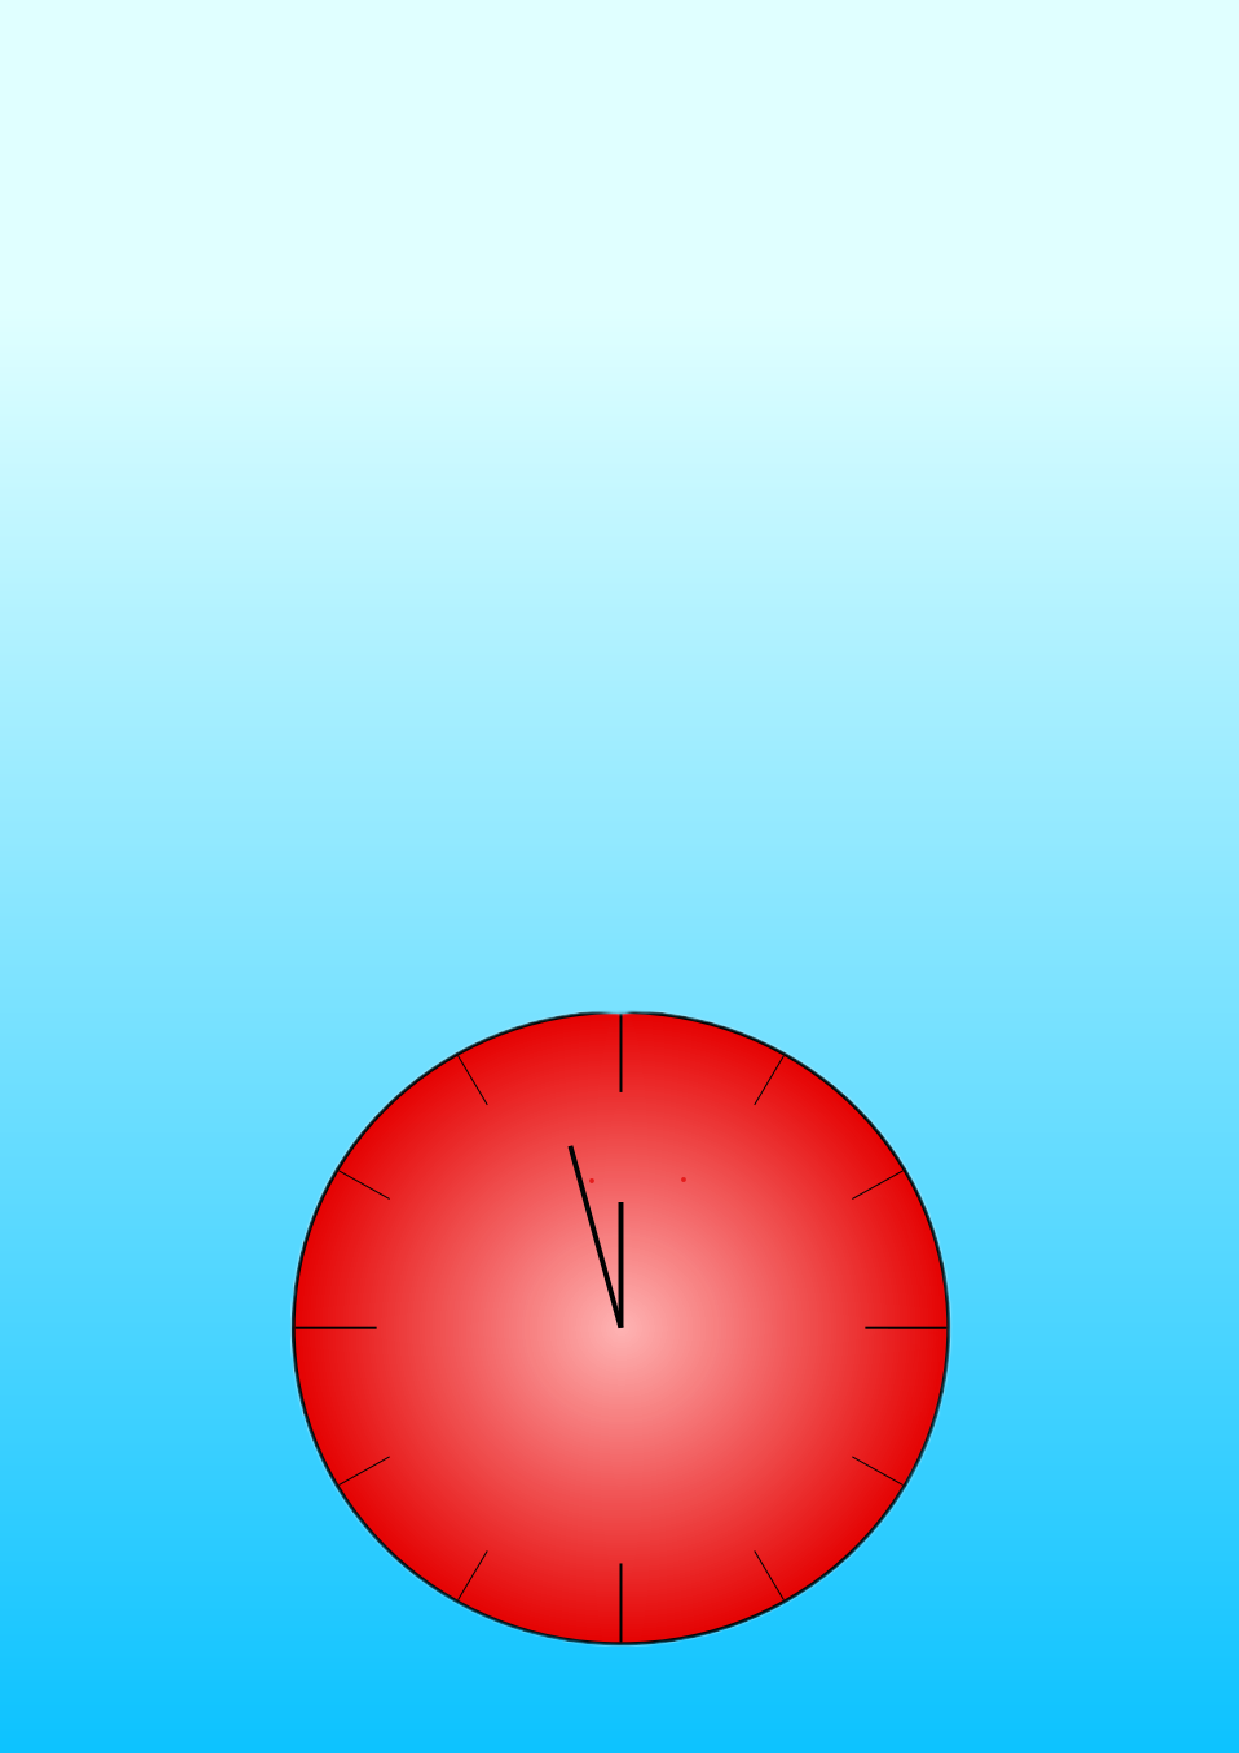
\includegraphics[height=\paperheight,width=\paperwidth]{img/pg}};
	%\tikz[remember picture,overlay] \fill[game] (current page.north west) rectangle (current page.south east); 
}
%
% sample boxes 
% 
\tcbset{
        framedbox/.style={
					enhanced, fontupper=\large,left=.75cm,fonttitle=\LARGE,toptitle=.25cm,bottomtitle=.25cm,halign title=center
        },
}

\newtcolorbox{basebox}[3][]{framedbox,coltitle=#2,colback=#3,coltext=#2,title=#1,colframe=#3,sharp corners}
\newtcolorbox{baseroundedbox}[3][]{framedbox,colback=#3,colframe=#3,coltitle=#2,coltext=#2,title=#1,,rounded corners,arc=15pt}
\newtcolorbox{transparentbox}[4][]{framedbox, colback=#3,colbacktitle=#3,colframe=#3,coltitle=#2,coltext=#2,title=#1,frame style={color=#3},opacitybacktitle=#4,opacityback=#4,opacityframe=#4,opacityfill=#4}
\newtcolorbox{blankbox}[1][]{blanker,fontupper=\LARGE,fonttitle=\bf\huge,title=#1,coltitle=black,top=.85cm}


% draw a grid
%\beamertemplategridbackground[0cm]

	\newcommand{\clock}[3]{%
		\begin{scope}[scale=14]
			\shadedraw [inner color=#1!30!white, outer color=#1!90!black, line width=12pt] (0,0) circle (1cm); 
			\foreach \angle in {0, 30, ..., 330} 
			\draw[line width=2pt] (\angle:0.82cm) -- (\angle:1cm);
			\foreach \angle in {0,90,180,270}
			\draw[line width=4pt] (\angle:0.75cm) -- (\angle:1cm);
			\draw[line width=8pt] (0,0) -- (90-270*#3:0.4cm);  
			\draw[line width=8pt] (0,0) -- (90-240*#3:0.6cm);  
		\end{scope}
	}


\begin{document}

\begin{frame}

	\begin{textblock}{45}(2,1)
		\begin{blankbox}
			
\includegraphics[width=1000pt]{img/gamename.png}
		\end{blankbox}
	\end{textblock}


	\begin{textblock}{75}[.5,.5](50,66)
		\centering
	
\begin{tikzpicture}

		\clock{red}{12}{11.5}

	\end{tikzpicture}
\end{textblock}

\begin{textblock}{35}(1,45)
		\begin{blankbox}[Brief Game Instructions]

			\begin{itemize}
							\item \textbf {Local CP}
							\item Health Threat Drop: People infected in an area -- rise after good decisions
							\item \textbf {Global CP}
							\item Citizen Trust: The faith citizens have on player -- rise after good decisions
							\item External Safety: Safety of the areas you govern -- drop after bad decisions
							\item Disposable Money: Financial support for fighting virus -- drop after bad decisions
						\end{itemize}
			
		\end{blankbox}
	\end{textblock}



	\begin{textblock}{20}(71,3.8)
		\begin{blankbox}
			\Huge\textbf{MINIMALISM}

\vspace{0.4cm}

			\textbf{SIMPLICITY}
\vspace{0.4cm}

\textbf{ENTERTAINMENT}
		\end{blankbox}
	\end{textblock}


	\begin{textblock}{40}(58,16)
		\begin{blankbox}[The clock is ticking!]


Lives are at stake, you need to take fast decisions to balance the safety of all the districts under your care!To terminate the virus, transfer the Critical Resources (CR) including doctors, medicine and other resources for fighting pandemic, between different areas to save them. Different CR has different effects in each area, your goal is to find the most effectively way of CR's distribution, in order to maintain your Control Points (CP) above 0, which indicates the situation of your administration and the pandemic. When all CP can be maintained above 0 for 5 minutes, you will terminate the pandemic! While any of your CP hitting 0,the pandemic beats you! Good luck! 

%Out of humanistic trans-regional assistance, the players, more often than not, are pressed to make moral decisions balancing the safety of districts by transferring Critical Resources (CR) lightning fast. Maintaining the regional Control Points (CP) above 0 in certain durations leads to victory. Alternatively, any CPs hitting 0 would instantly indicate failure.\vspace {0.4cm}

% Terminator recreates for the players the scenario where countless medical workers, policy makers and all the other concerned parties had to make tough decisions facing extremelystressful situations just to save our lives and protect our countries as best as they can during the real pandemic COVID-19 last year. May their great spirit inspire us.
		\end{blankbox}
	\end{textblock}



	% #1: box width 
	% #2 #3: coordinates on percent 


	
	\begin{textblock}{50}(25,70)
		% no title provided, extra parameter is opacity in [0,1] 		
		\begin{transparentbox}{black}{red}{.2}
				\centering \vspace{.55cm}
				\huge\textbf{Developer's philosophy}\vspace{1cm}

\begin{itemize}\itemsep .85cm
				\item \textbf{Easy and intuitive control} 

				\item \textbf{Simplism User Interface}

				\item  \textbf{Self-made mods} 

				\item  \textbf{Cross-platform game} 
\end{itemize}       	 



		\end{transparentbox}
	\end{textblock} 

	% option [0,1] means box anchor is bottom left	





	\begin{textblock}{30}(28,92)
		\begin{blankbox}
			
\includegraphics[width=200pt]{img/Teamlogo.png}

		\end{blankbox}
	\end{textblock}


	\begin{textblock}{80}[0,1](1,100)
		 
			
\includegraphics[width=195pt]{img/JI-dark.pdf}
	\end{textblock}

	\begin{textblock}{10}(14,92)
		\begin{blankbox}
			\centering
			
\includegraphics[height=190pt]{img/SF-head.pdf}
		\end{blankbox}
	\end{textblock}

	% option [1,1] means box anchor is bottom right	
	\begin{textblock}{52}[1,1](100,100)
			\huge\textbf{{Three To One:}} Zining Wang (C), Yifan Jia, Qiao Liu
	\end{textblock}

	\begin{textblock}{52}[.5,.5](50,89.5)

		\centering\em\bf\Huge
			The current pandemic inspired this game. 

			Become a protagonist and a savior!

	\end{textblock}
	\begin{textblock}{10}(7,70)
		\begin{blankbox}
			\centering
			
\includegraphics[height=400pt]{img/ai97b-ej97b.png}
		\end{blankbox}
	\end{textblock}

	\begin{textblock}{10}(80,70)
		\begin{blankbox}
			\centering
			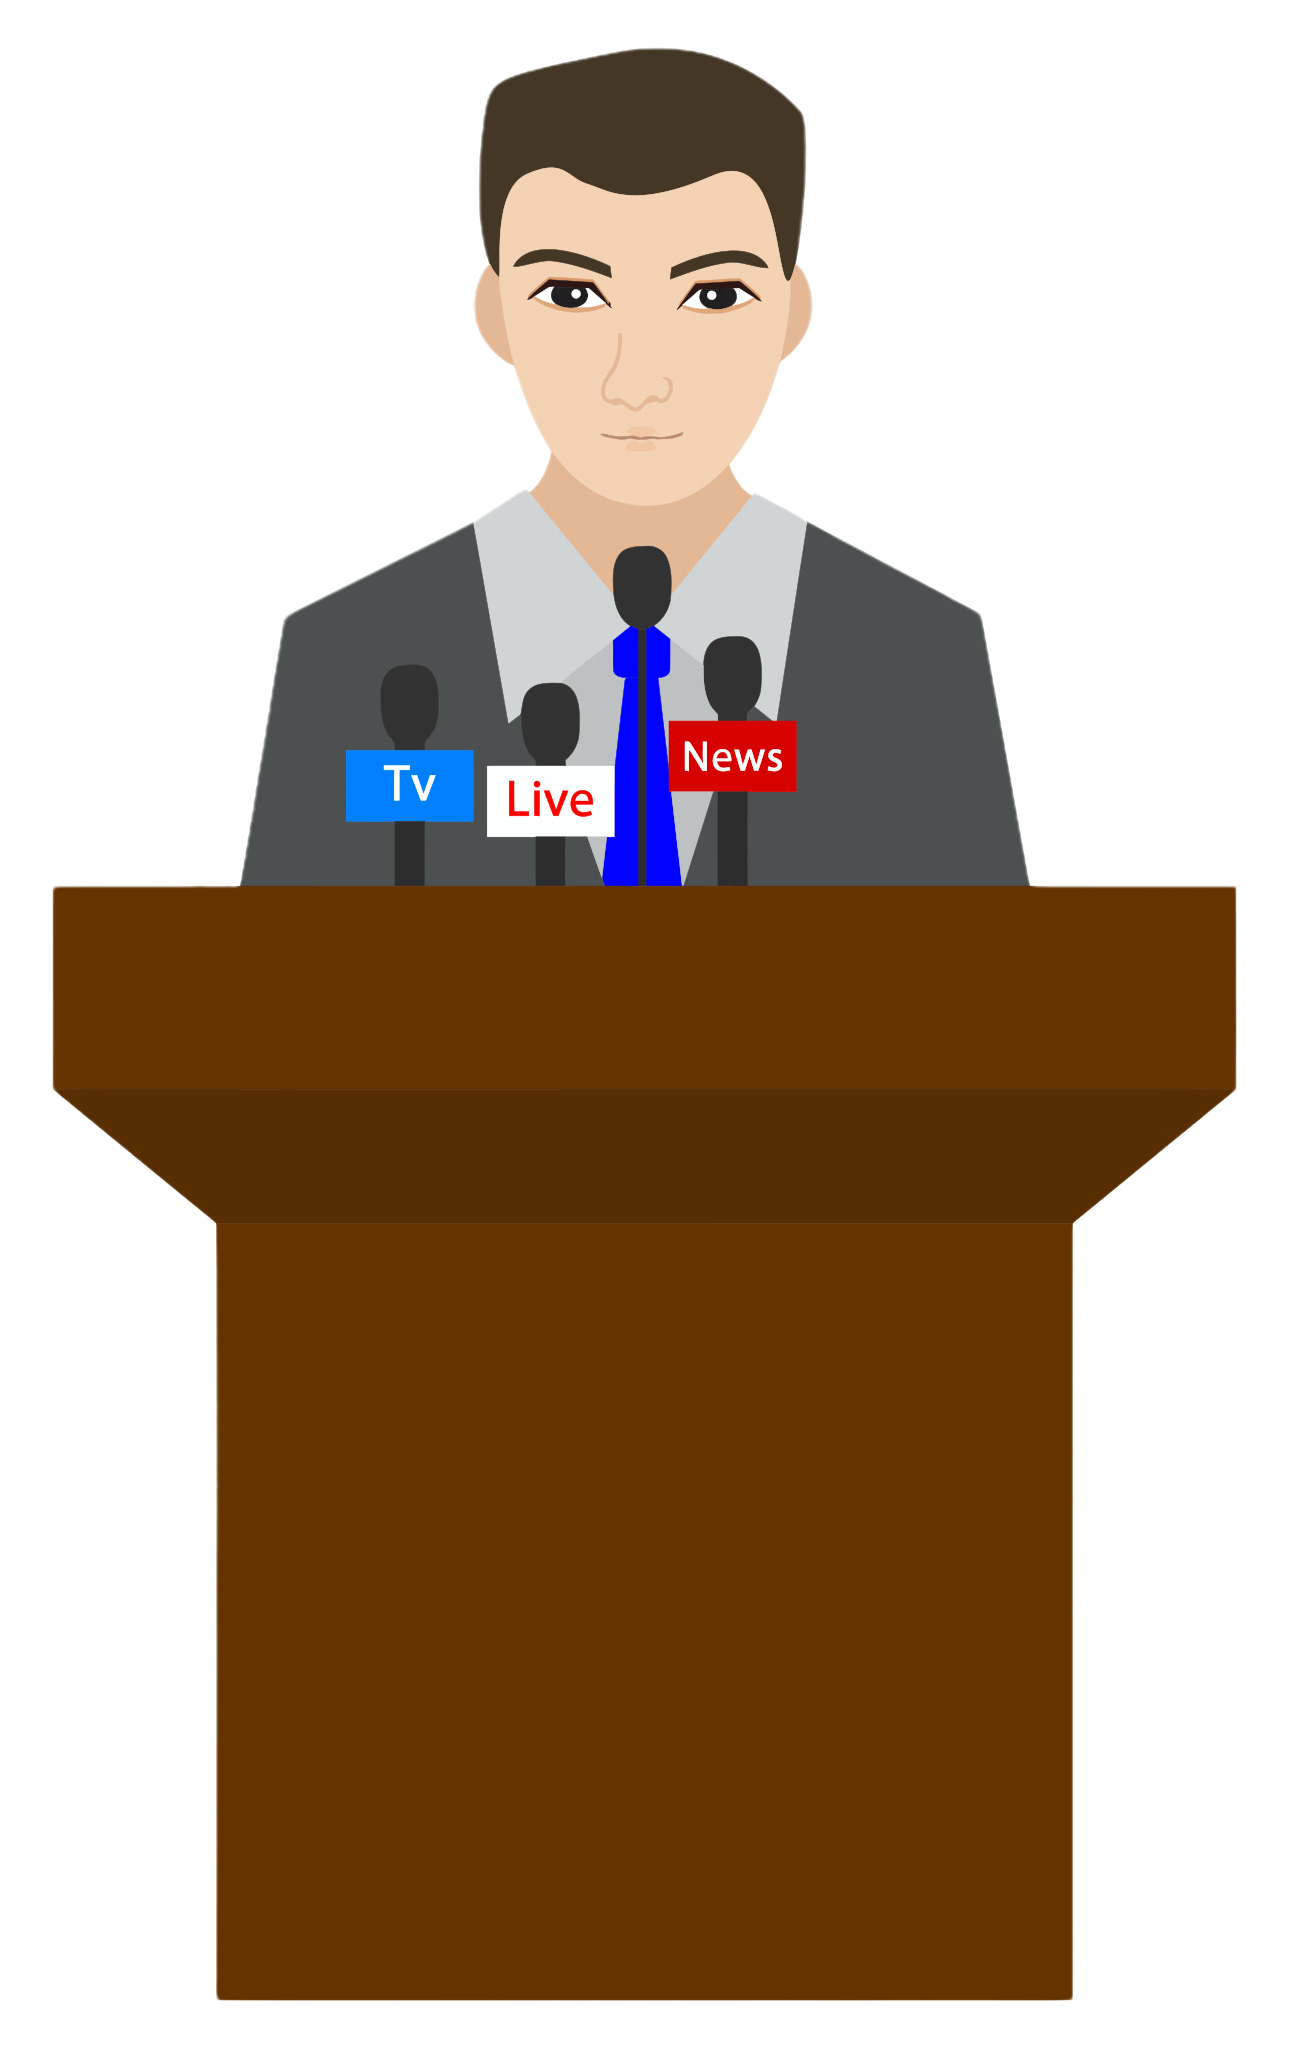
\includegraphics[height=400pt]{img/arn28-kj5eh.png}
		\end{blankbox}
	\end{textblock}

	\begin{textblock}{40}(38,42)
		\begin{blankbox}
			\centering
			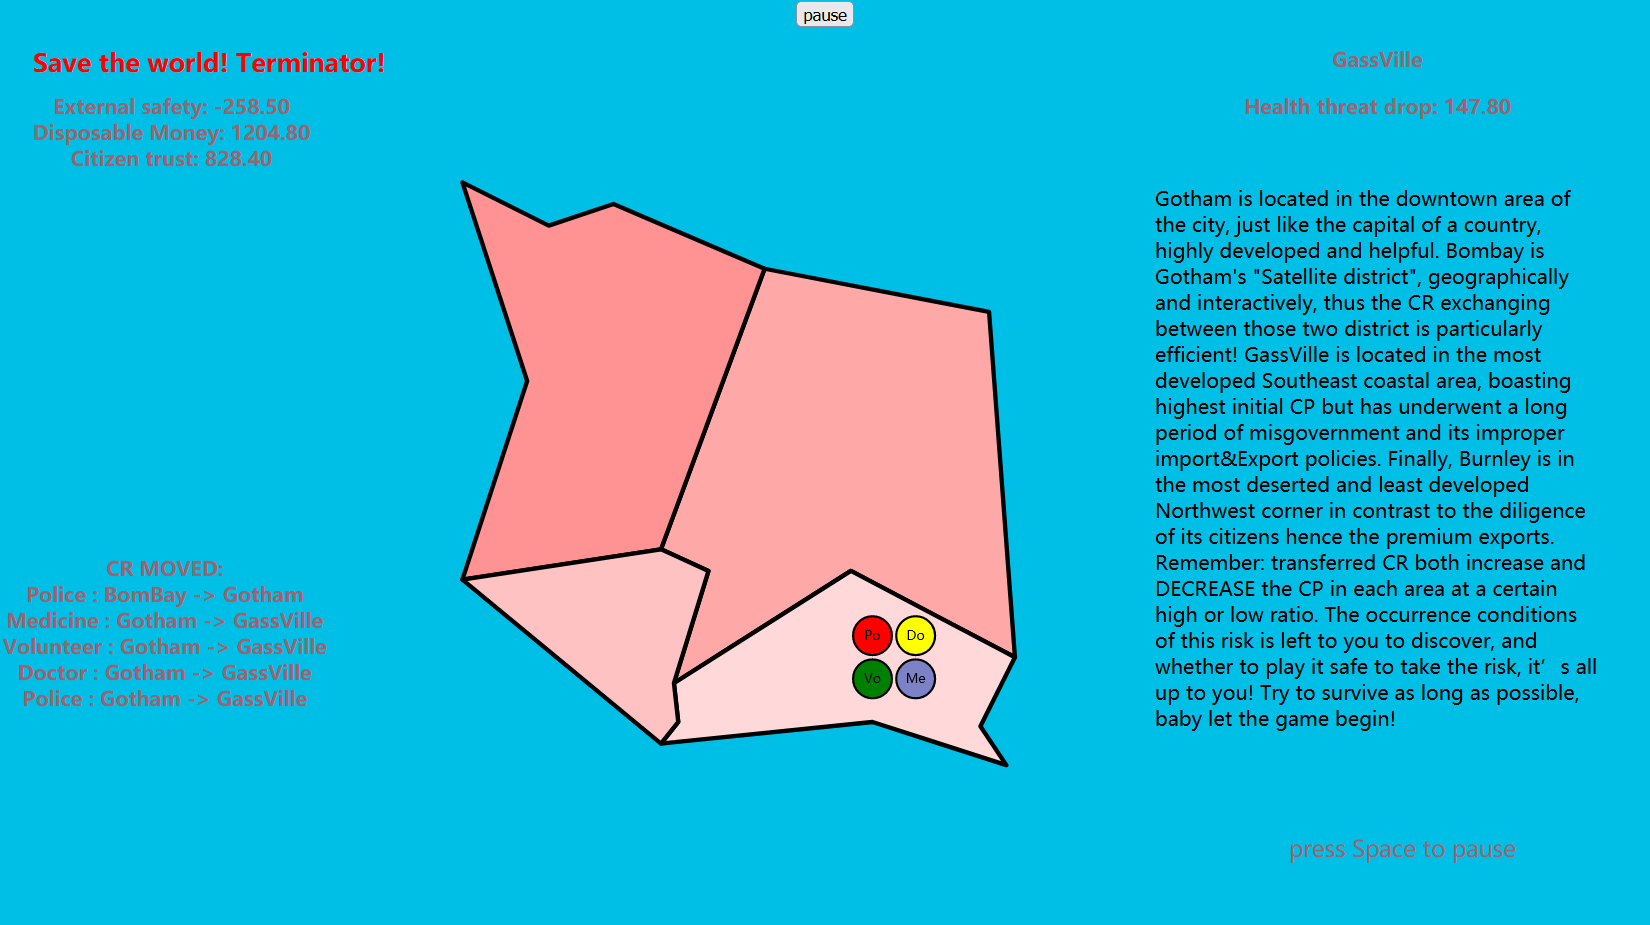
\includegraphics[ height=570pt]{img/newDemo}
		\end{blankbox}
	\end{textblock}
\begin{turn}{60}
	\begin{textblock}{1}(67,3)
		\begin{blankbox}
			\centering
			
\includegraphics[height=200pt]{img/aLine}
		\end{blankbox}
	\end{textblock}
\end{turn}


	\begin{textblock}{9}(0.5,15)
		\begin{blankbox}
			\centering
			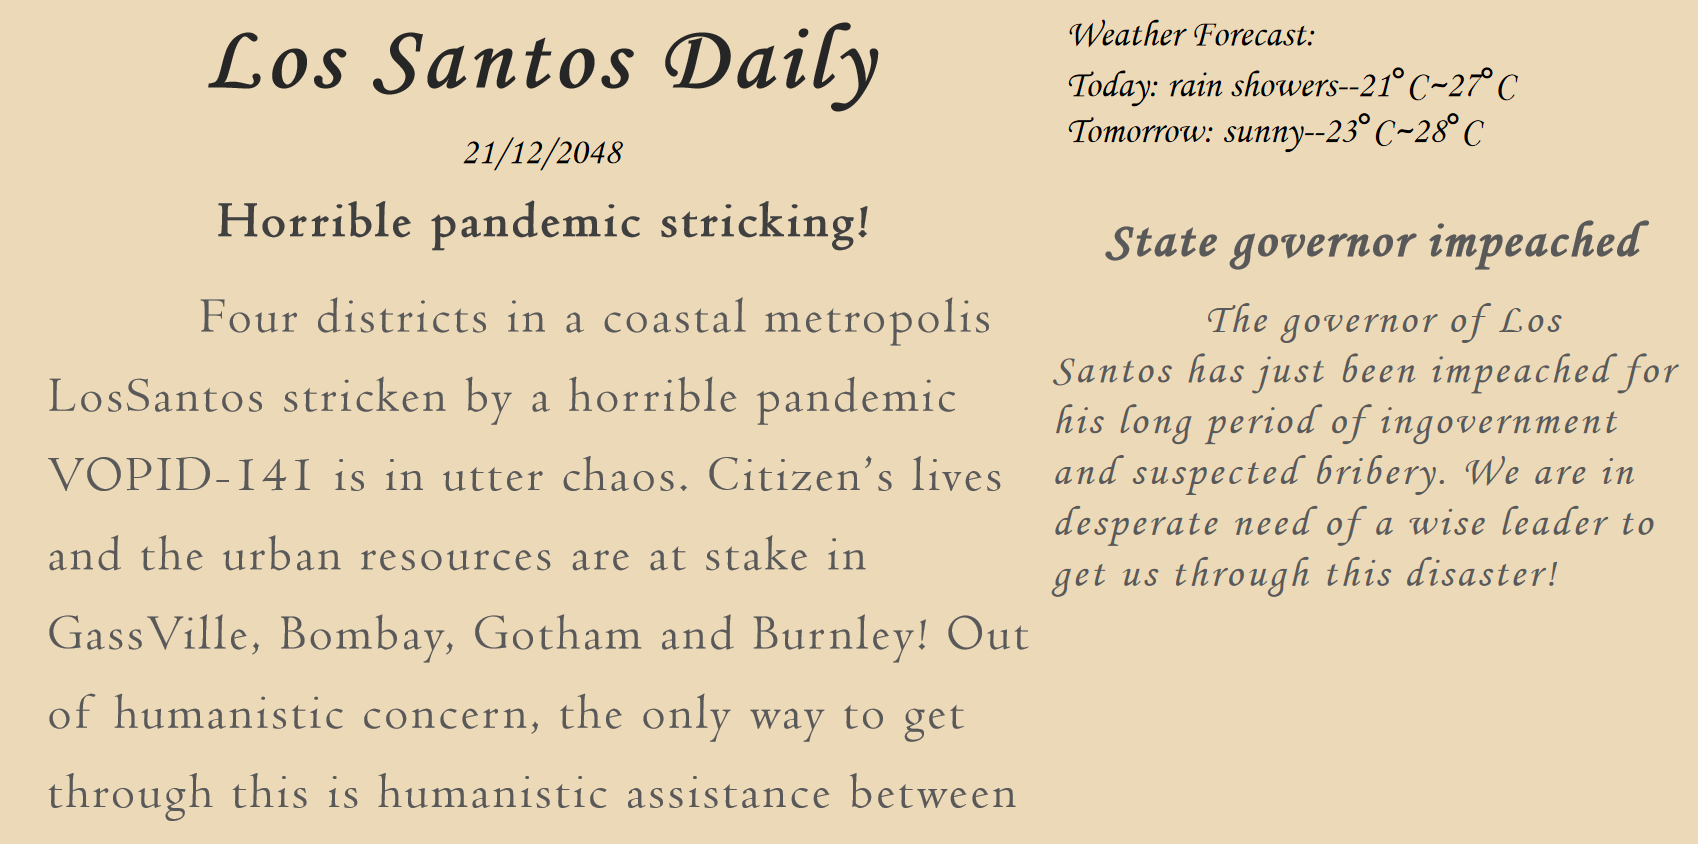
\includegraphics[angle=8,height=550pt]{img/news.png}
		\end{blankbox}
	\end{textblock}


\end{frame}

\end{document}